%%%%%%%%%%%%%%%%%%%%%%%%%%%%%%%%%%%%%%%%%
% Lachaise Assignment
% LaTeX Template
% Version 1.0 (26/6/2018)
%
% This template originates from:
% http://www.LaTeXTemplates.com
%
% Authors:
% Marion Lachaise & François Févotte
% Vel (vel@LaTeXTemplates.com)
%
% License:
% CC BY-NC-SA 3.0 (http://creativecommons.org/licenses/by-nc-sa/3.0/)
% 
%%%%%%%%%%%%%%%%%%%%%%%%%%%%%%%%%%%%%%%%%

%----------------------------------------------------------------------------------------
%	PACKAGES AND OTHER DOCUMENT CONFIGURATIONS
%----------------------------------------------------------------------------------------

\documentclass{article}

\input{structure.tex} % Include the file specifying the document structure and custom commands

%----------------------------------------------------------------------------------------
%	ASSIGNMENT INFORMATION
%----------------------------------------------------------------------------------------

\title{MAE001: Modelagem Matemática em Finanças I} % Title of the assignment
\date{Universidade Federal do Rio de Janeiro (UFRJ) --- \today} % University, school and/or department name(s) and a date

\author{Ramon Duarte de Melo\\ \texttt{ramonduarte@poli.ufrj.br} % Author name and email address
\\ \\ Alex Teixeira da Silva\\ \texttt{alextx@poli.ufrj.br}} % Author name and email address



%----------------------------------------------------------------------------------------

\begin{document}

\maketitle % Print the title

%----------------------------------------------------------------------------------------
%	INTRODUCTION
%----------------------------------------------------------------------------------------

\section*{Introdução} % Unnumbered section

O objetivo do Projeto 4 é implementar, avaliar e comparar o modelo do \emph{Capital Asset Pricing Model} com os dados fornecidos pelo mundo real, realizando comparações de estruturas de termo e produzindo gráficos com tais observações. 

Para tal, foi utilizada a linguagem \emph{Python 3.6.7}, com os módulos \emph{numpy} (métodos numéricos), \emph{pandas} (manipulação de dados), \emph{scipy} (fórmulas científicas) e \emph{matplotlib.pyplot} (visualização de dados). Um arquivo \texttt{Pipenv} foi disponibilizado para instalar as dependências de forma automatizada.

Os dados utilizados para a confecção dos gráficos foram obtidos através do site do Tesouro Nacional (\textsl{tesouro.gov.br}), do site da B3 S.A, operadora da Bolsa de Valores de São Paulo (\textsf{}), e da \emph{API} do Yahoo Finance (\textsl{}). Os procedimentos de execução estão descritos em arquivos \texttt{.ipynb}, que requerem o módulo \emph{Jupyter Notebook} para ser executado.


O código utilizado neste trabalho, bem como o deste relatório e as imagens geradas, foi aberto e disponibilizado publicamente no repositório https://github.com/ramonduarte/mmftrab4.


%----------------------------------------------------------------------------------------
%	PROBLEM 1
%----------------------------------------------------------------------------------------

\section*{Atividade \emph{1}} % Numbered section

Nesta atividade, a estrutura a termo da taxa de juros de títulos prefixados do Tesouro Nacional (\emph{LTNs}, sem prêmios semestrais) foi adquirida da web e dela extraída a taxa de juros dos anos de 2016, 2017 e 2018 para os próximos 6 a 7 anos.

Como alguns títulos não são emitidos no início do ano (sobretudo os de mais longa duração até o exercício), as datas foram padronizadas para o mesmo dia em cada ano, 2º de fevereiro.
A escolha por esta data deu-se por ser o primeiro dia útil onde todos os títulos foram disponibilizados.

Os arquivos foram obtidos em formato \texttt{.xls} (padrão Microsoft Excel 2003), parseados e plotados em gráficos $t \times r$.
Para cada gráfico, uma curva \emph{spline} cúbica que perpassa todos os pontos também foi plotada.
A opção pela \emph{spline} cúbica é devido a, além de ser a mais popular, ser a melhor curva possível para para o baixo número de pontos de dados disponíveis (entre quatro e cinco).


\begin{figure}[H]
	\includegraphics[width=0.6\linewidth]{Figure_0.png}
	\centering
	
	\caption{Gráfico $t \times r$ para ativos \textbf{LTN} com data de emissão 02/02/2016.}
	\label{}
\end{figure}

\begin{figure}[]
	\includegraphics[width=0.6\linewidth]{Figure_1.png}
	\centering
	
	\caption{Gráfico $t \times r$ para ativos \textbf{LTN} com data de emissão 02/02/2017.}
	\label{}
\end{figure}

\begin{figure}[]
	\includegraphics[width=0.6\linewidth]{Figure_2.png}
	\centering
	
	\caption{Gráfico $t \times r$ para ativos \textbf{LTN} com data de emissão 02/02/2018.}
	\label{}
\end{figure}

%----------------------------------------------------------------------------------------
%	PROBLEM 2
%----------------------------------------------------------------------------------------


\section*{Atividade \emph{2}}

Para esta atividade, os dados utilizados foram os mesmos dos da anterior, de forma que a aquisição e a organização deles foi análoga.
As ferramentas utilizadas também foram as mesmas.

Porém, aqui se deseja avaliar o valor dos títulos prefixados através de predição, utilizando o modelo de Ho-Lee.
Portanto, os dados foram agrupados pelo intervalo entre a aquisição e a data de exercício, ao contrário da atividade anterior, em que eram agregados por ano de emissão.

Os dados utilizados foram a distribuição das taxas diárias (\emph{intraday} de juros negociadas nos títulos (chamada de $r(t)$) e o preço unitário de cada título (chamado de $up_{t}$.
Desta forma, as predições foram calculadas de acordo com o modelo:

\begin{equation}
	d r(t) = \theta (t) dt + \sigma dW(t)
\end{equation}

onde $\theta$ é o valor esperado do título no momento de exercício, $\sigma$ é o desvio-padrão da distribuição de taxas de juros, e $dW(t)$ é a distribuição de variações diárias de $r(t)$.

O modelo foi calculado de acordo com os seguintes parâmetros:

\begin{equation}
	\theta (t) = u_{p}(t) (1 + r(t))
\end{equation}

\begin{equation}
	d W(t) = r(t) - r(t - 1)
\end{equation}

Cada gráfico possui uma duração até o prazo de exercício fixada e tem os dados espalhados (\emph{scatter plot})na forma $t \times r(t)$. 
Foram selecionados 36 datas para cada domínio, representando os doze meses ao longo dos três anos analisados.
Cada estrutura a termo também foi interpolado por uma \emph{spline} cúbica ou acrescido de uma reta de regressão linear. 


\begin{figure}[H]
	\includegraphics[width=0.6\linewidth]{Figure_3.png}
	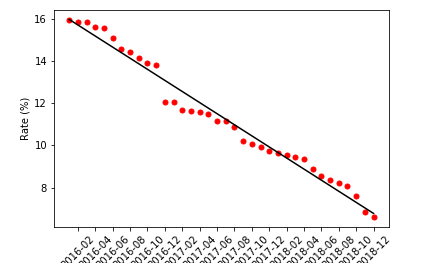
\includegraphics[width=0.6\linewidth]{Figure_4.png}
	\centering
	
	\caption{Gráfico $t \times r$ para ativos \textbf{LTN} com prazos de exercício de 12 meses.}
	\label{}
\end{figure}

\begin{figure}[H]
	\includegraphics[width=0.6\linewidth]{Figure_5.png}
	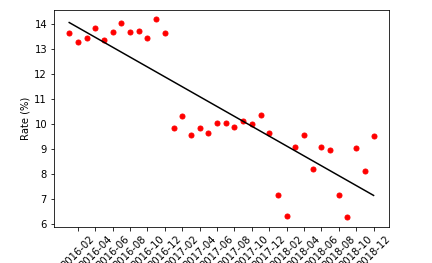
\includegraphics[width=0.6\linewidth]{Figure_6.png}
	\centering
	
	\caption{Gráfico $t \times r$ para ativos \textbf{LTN} com prazos de exercício de 24 meses.}
	\label{}
\end{figure}

\begin{figure}[H]
	\includegraphics[width=0.6\linewidth]{Figure_7.png}
	\centering
	
	\caption{Gráfico $t \times r$ para ativos \textbf{LTN} com prazos de exercício de 60 meses.}
	\label{}
\end{figure}

\begin{figure}[H]
	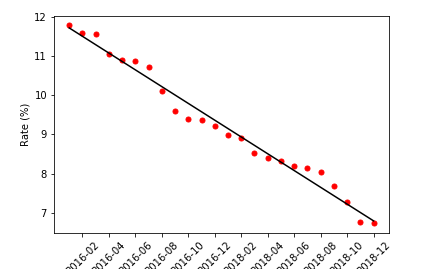
\includegraphics[width=0.6\linewidth]{Figure_8.png}
	\centering
	
	\caption{Gráfico $t \times r$ para ativos \textbf{LTN} com prazos de exercício de 60 meses.}
	\label{}
\end{figure}


%----------------------------------------------------------------------------------------
%	PROBLEM 2
%----------------------------------------------------------------------------------------

\section*{Atividade c}

Por fim, deseja-se estudar o modelo CAPM e do portfólio moderno com base em ações razoavelmente negociadas na Bolsa de Valores.
Quatro ativos de empresas de setores distintos foram escolhidos: ABEV3 (Ambev S.A.), CIEL3 (Cielo S.A.), ITUB4 (Itaú Unibanco Holding S.A.) e PETR4 (Petróleo Brasileiro S.A.).
Todos os ativos estão listados pela B3 no IBOVESPA, que reúne os 500 ativos mais negociados na Bolsa de Valores de São Paulo. 

Os dados utilizados foram coletados da API do \emph{Yahoo Finance}.
Por conta disso, não houve a necessidade de raspar ou tratar os dados.

\begin{table}[H]
	\centering
	\begin{tabular}{llllll}
	 & \textbf{PETR4.SA} & \textbf{ABEV3.SA} & \textbf{CIEL3.SA} & \textbf{ITUB4.SA} & \textbf{\^{}BVSP} \\
	\textbf{PETR4.SA} & 0.229935 & 0.032758 & 0.042141 & 0.086051 & 0.083885 \\
	\textbf{ABEV3.SA} & 0.032758 & 0.052819 & 0.021265 & 0.026578 & 0.024687 \\
	\textbf{CIEL3.SA} & 0.042141 & 0.021265 & 0.106951 & 0.031632 & 0.029463 \\
	\textbf{ITUB4.SA} & 0.086051 & 0.106951 & 0.031632 & 0.092219 & 0.055982 \\
	\textbf{\^{}BVSP} & 0.083885 & 0.024687 & 0.029463 & 0.055982 & 0.050850
	\end{tabular}
	\caption{Matriz de covariância das ações. IBOVESPA adicionado como referência.}
	\label{tab:my-table}
\end{table}

Baseado neles, calculou-se o índice Sharpe, a matriz de covariância e o valor esperado do retorno sobre investimento anualizado.
Foram construídos dois portfólios, um com objetivo de atingir 6,7\% em 12 meses e o outro, 7,0\% no mesmo tempo.
Para cada um deles, foi escolhido uma porção de cada ativo de forma a minimizar o risco, aqui medido como o desvio padrão das séries históricas. 


\begin{table}[H]
	\centering
	\begin{tabular}{lll}
	 & \textbf{Índice Sharpe.}& \textbf{Retorno esp.} \\
	\textbf{PETR4.SA} & 0.229935 & 0.071282 \\
	\textbf{ABEV3.SA} & 0.032758 & 0.066849 \\
	\textbf{CIEL3.SA} & 0.042141 & 0.067206 \\
	\textbf{ITUB4.SA} & 0.086051 & 0.069193 \\
	\textbf{Portfólio 1} & 0.094948 & 0.067000 \\
	\textbf{Portfólio 2} & 0.012713 & 0.700000 \\
	\textbf{\^{}BVSP} & 0.083885 & 0.068808
	\end{tabular}
	\caption{Índice Sharpe e esperança da taxa de retorno.}
	\label{tab:my-table}
\end{table}


\end{document}
